\documentclass[11pt,a4paper]{article} 

\usepackage{titlesec}
\usepackage{color}
\usepackage[utf8]{inputenc}
\usepackage[english]{babel}
\usepackage[T1]{fontenc}
\usepackage{graphicx}
\graphicspath{{Images/}}
\usepackage{eso-pic} 
\usepackage{subfig} 
\usepackage{caption}
\usepackage{transparent}

% STANDARD MATH PACKAGES
\usepackage{amsmath}
\usepackage{amsthm}
\usepackage{bm}
\usepackage[overload]{empheq} 

% PACKAGES FOR TABLES
\usepackage{tabularx}
\usepackage{colortbl}

% PACKAGES FOR ALGORITHMS (PSEUDO-CODE)
\usepackage{algorithm}
\usepackage{algorithmic}

% PACKAGES FOR REFERENCES & BIBLIOGRAPHY
\usepackage[colorlinks=true,linkcolor=black,anchorcolor=black,citecolor=black,filecolor=black,menucolor=black,runcolor=black,urlcolor=black]{hyperref} % Adds clickable links at references
\usepackage{cleveref}
\usepackage[square, numbers, sort&compress]{natbib} 

% PACKAGES FOR THE APPENDIX
\usepackage{appendix}

% PACKAGES FOR ITEMIZE & ENUMERATES 
\usepackage{enumitem}

% OTHER PACKAGES
\usepackage{amsthm,thmtools,xcolor} % Coloured "Theorem"
\usepackage{fancyhdr} % Fancy headers and footers
\usepackage{lipsum} % Insert dummy text
\usepackage{tcolorbox} % Create coloured boxes
\usepackage{graphicx}




% Do not change Configuration_files/config.tex file unless you really know what you are doing.
%DO NOT EDIT
% Configuration package
\usepackage[bottom=2.0cm,top=2.0cm,left=2.0cm,right=2.0cm]{geometry}
\raggedbottom 

\definecolor{newblue}{cmyk}{0.4,0.1,0,0.4}

% Custom theorem environments
\declaretheoremstyle[
  headfont=\color{newblue}\normalfont\bfseries,
  bodyfont=\color{black}\normalfont\itshape,
]{colored}

\captionsetup[figure]{labelfont={color=newblue}} 
\captionsetup[table]{labelfont={color=newblue}} 
\captionsetup[algorithm]{labelfont={color=newblue}} 

\theoremstyle{colored}
\newtheorem{theorem}{Theorem}[section]
\newtheorem{proposition}{Proposition}[section]

\newcommand\T{\rule{0pt}{2.6ex}}
\newcommand\B{\rule[-1.2ex]{0pt}{0pt}}

\newcounter{algsubstate}
\renewcommand{\thealgsubstate}{\alph{algsubstate}}
\newenvironment{algsubstates}{
    \setcounter{algsubstate}{0}%
    \renewcommand{\STATE}{%
    \stepcounter{algsubstate}%
    \Statex {\small\thealgsubstate:}\space}
    }{}
    
% Custom theorem environment
\newcolumntype{L}[1]{>{\raggedright\let\newline\\\arraybackslash\hspace{0pt}}m{#1}}
\newcolumntype{C}[1]{>{\centering\let\newline\\\arraybackslash\hspace{0pt}}m{#1}}
\newcolumntype{R}[1]{>{\raggedleft\let\newline\\\arraybackslash\hspace{0pt}}m{#1}}

% Custom itemize environment
\setlist[itemize,1]{label=$\bullet$}
\setlist[itemize,2]{label=$\circ$}
\setlist[itemize,3]{label=$-$}
\setlist{nosep}


\setlength\parindent{0pt}

% Custom title commands
\titleformat{\section}
{\color{newblue}\normalfont\Large\bfseries}
{\color{newblue}\thesection.}{1em}{}
\titlespacing*{\section}
{0pt}{3.3ex}{3.3ex}

\titleformat{\subsection}
{\color{newblue}\normalfont\large\bfseries}
{\color{newblue}\thesubsection.}{1em}{}
\titlespacing*{\subsection}
{0pt}{3.3ex}{3.3ex}

% Custom headers and footers
\pagestyle{fancy}
\fancyhf{}
      
\fancyfoot{}
\fancyfoot[C]{\thepage} % page
\renewcommand{\headrulewidth}{0mm} % headrule width
\renewcommand{\footrulewidth}{0mm} % footrule width

\makeatletter
\patchcmd{\headrule}{\hrule}{\color{black}\hrule}{}{} % headrule
\patchcmd{\footrule}{\hrule}{\color{black}\hrule}{}{} % footrule
\makeatother

\renewcommand{\title}{Efficient Text Searching}
\newcommand{\authorA}{Abhijeet Singh 2023CSB1094}
\newcommand{\authorB}{Parashdeep Singh 2023MCB1306}
\newcommand{\authorC}{Aadit Mahajan 2023CSB1091} 

\newcommand{\advisor}{Dr. Anil Shukla}
\newcommand{\firstcoadvisor}{Sravanthi Shede}
\newcommand{\summary}{We have used data structures like Tries and Suffix Trees, and algorithms like KMP and Finite Automata algorithms to perform pattern searching in a text file. Our code basically gives the output of the line of occurrence of searched pattern and the pattern's starting index in that line. As we are using these various methods to perform pattern searching, so we have done complexity analysis for all the methods in order to determine which method is optimal.}

%-------------------------------------------------------------------------
%	BEGIN OF YOUR DOCUMENT
%-------------------------------------------------------------------------
\begin{document}

% Do not change Configuration_files/TitlePage.tex
% DO NOT EDIT

\null\hfill
\includegraphics[width=0.2\textwidth]{logo.jpg}

\vspace{3mm}
\Large{\textbf{\color{newblue}{\title}}}
\vspace{0.1cm}\\
\large{\textbf{\authorA}}\vspace{1mm}
,\\ \large{\textbf{\authorB}}\vspace{1mm}
\ifdefined \authorC
,\\ \large{\textbf{\authorC}}\vspace{1mm}
\ifdefined \authorD
,\\ \large{\textbf{\authorD}}\vspace{1mm}
\fi 
\fi
\small \normalfont

\vspace{11pt}

\centerline{\rule{1.0\textwidth}{0.4pt}}

\begin{center}
\begin{minipage}[t]{.24\textwidth}
\begin{minipage}{.90\textwidth}
\noindent
\footnotesize{\textbf{Course Instructor:} \\
\advisor} \\
\\
\footnotesize{\textbf{TA :}\\ 
\firstcoadvisor}\\ 

\end{minipage}
\end{minipage}
\begin{minipage}{.74\textwidth}
\noindent \textbf{\color{red} Overview:} {\summary}
\end{minipage}
\end{center}

\vspace{8pt}

\centerline{\rule{1.0\textwidth}{0.4pt}}
\vspace{12pt}
%Main Text starting point
\section{Trie and Suffix Tree}
\textbf{Trie}
\label{sec:introduction}
\\
The \textbf{\textbf{Trie data structure}} is a tree-like data structure used for storing a dynamic set of strings. It is commonly used for efficient \textbf{\textbf{retrieval }}and \textbf{\textbf{storage }}of keys in a large dataset. The structure supports operations such as \textbf{\textbf{insertion}}, \textbf{\textbf{search}}, and \textbf{\textbf{deletion }}of keys, making it a valuable tool in fields like computer science and information retrieval. They are particularly useful when we have a large number of strings with significant overlap in their prefixes.
\\
\\
\textbf{Properties:} 1. It contains a single root node.
\\
2. Each node represents a string and each edge represents a character.
\\
3. Every node consists of an array of pointers, with each index representing a character and a flag to indicate if any string ends at the current node.
\\
4. Although, trie data structure can contain any number of characters including alphabets, numbers, and special characters but here we only need 26 pointers for every node, where the 0th index represents ‘a’ and the 25th index represents ‘z’ characters.
\\
5. Each path from the root to any node represents a word or string.
\\

\subsection{Construction Of Trie}

\subsubsection{Representation of Trie Node}
Every Trie node consists of a character pointer array or hashmap and a flag to represent if the word is ending at that node or not. But if the words contain only lower-case letters (i.e. a-z), then we can define Trie Node with an array instead of a hashmap.
\begin{algorithm}[H]
\caption*{Representation of Trie Node}
\label{TrieNodepsuedocode}
\begin{algorithmic}
\STATE Constructing a trie node, 
\STATE \hspace{0.3cm} struct TrieNode
\STATE \hspace{1cm} TrieNode *children[26];
\STATE \hspace{1cm} bool isEndOfWord;
\end{algorithmic}
\end{algorithm}
\begin{algorithm}[H]
\begin{algorithmic}
\caption*{Creating a new Trie Node}
\STATE Initializing a trie node, 
\STATE \hspace{0.3cm} struct TrieNode* node;
\STATE \hspace{0.3cm} node->isEndOfWord=false;
\STATE \hspace{0.3cm} for i in range(26):
\STATE \hspace{1cm} node->children[i]=NULL   
\end{algorithmic}
\end{algorithm}

\subsubsection{Insertion in Trie}
\label{subsec:naiveInsertionalgorithm}
\paragraph{Algorithm}
1. Define a function insert(TrieNode *root, string &word) which will take two parameters one for the root and the other for the string that we want to insert in the Trie data structure.
\\
2. Now take another pointer currentNode and initialize it with the root node.
\\
3. Iterate over the length of the given string and check if the value is NULL or not in the array of pointers at the current character of the string.
\\
4. If It’s NULL then, make a new node and point the current character to this newly created node. Move the currentNode pointer to the newly created node.
\\
5. Finally, change the flag value of "isEndOfWord" of the last currentNode to true, this implies that there is a string ending currentNode.
\\
\begin{algorithm}[H]
\caption*{Insertion in Trie \begin{math} ( \end{math} struct TrieNode *root, string key \begin{math} ) \end{math} }
\label{InsertionTriepsuedocode}
\begin{algorithmic}
\STATE struct TrieNode *node \begin{math} = \end{math} root;
\FOR{$1 \leq i \leq key.length$}
\STATE int index \begin{math}= key[i] - \end{math} 'a';
\IF{\begin{math} !node->children[index] \end{math}}
\STATE \hspace{0.5cm} \begin{math} node->children[index] = getNode() \end{math};
\ENDIF
\STATE \begin{math} node = node->children[index] \end{math}
\ENDFOR
\\
\begin{math} node->isEndofWord = true \end{math}
\end{algorithmic}
\end{algorithm}

For example, let us take a look at a trie and see how words are stored in it.

### 1. Store “and” in Trie data structure:

The word “and” starts with “a“, so we will mark the position “a” as filled in the Trie node, which represents the use of “a”. After placing the first character, for the second character, again there are 26 possibilities. So from “a“, there is an array of size 26 for storing the 2nd character. The second character is “n“, so from “a“, we move to “n” and mark “n” in the 2nd array as used. The third character is “d“, so we mark the position “d” as used in the respective array.


### 2. Store “ant” in the Trie data structure:

The word “ant” starts with “a”, and the position of “a” in the root node has already been filled. So, no need to fill it again; just move to the node ‘a‘ in the Trie.
For the second character ‘n‘, we observe that the position of ‘n’ in the ‘a’ node has already been filled. No need to fill it again; just move to the node ‘n’ in the Trie.
For the last character ‘t‘ of the word, the position for ‘t‘ in the ‘n‘ node is not filled. So, fill the position of ‘t‘ in the ‘n‘ node and move to the ‘t‘ node.

\begin{figure}[H]
    \centering
    % Uncomment the line below to include the image
    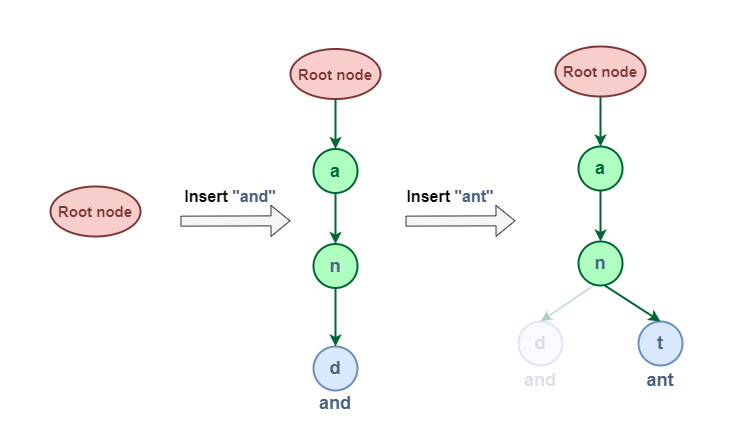
\includegraphics[width=14cm, height=10cm]{Triedatastructure1.png}
    \caption{Representation of how words are stored in Trie}
    \label{fig:StoringExample}
\end{figure}


\subsubsection{Searching in Trie}
\label{subsec:SearchingTrie}
Search operation in Trie is performed in a similar way as the insertion operation but the only difference is that whenever we find that the array of pointers in currentNode does not point to the current character of the word then we return false instead of creating a new node for that current character of the word. This operation is used to search whether a string is present in the Trie data structure or not. There are two search approaches in the Trie data structure.
\\
1. Find whether the given word exists in Trie.
\\
2. Find whether any word that starts with the given prefix exists in Trie.
\\
There is a similar search pattern in both approaches. The first step in searching a given word in Trie is to convert the word to characters and then compare every character with the trie node from the root node. If the current character is present in the node, move forward to its children. Repeat this process until all characters are found.

\\
\begin{algorithm}[H]
\caption*{Searching in Trie \begin{math} ( \end{math} struct TrieNode *root, string key \begin{math} ) \end{math}}
\label{DeletionTriepsuedocode}
\begin{algorithmic}
\STATE \textbf{Initialize:} struct TrieNode *node \begin{math} = \end{math} root
\FOR{$i = 0$ to $key.length - 1$}
    \STATE int index \begin{math} = \end{math} key[i] \begin{math} - \end{math} 'a'
    \IF{\begin{math} node \to children[index] = \text{NULL} \end{math}}
        \STATE \hspace{0.5cm} \textbf{return} false
    \ENDIF
    \STATE node \begin{math} = \end{math} node \to children[index]
\ENDFOR
\STATE \textbf{return} \begin{math} (node \to isEndOfWord) \end{math}
\end{algorithmic}
\end{algorithm}



\textbf{Time Complexity}
The time taken by this algorithm is \begin{math}O(n^2)\end{math} where 'n' is the length of the text. This time is essentially taken to build the trie. Note that this is one time activity and subsequent searches of another pattern in this text would take \begin{math} O(m) \end{math} time where m is the length of the pattern. \vspace{0.8 cm}

\textbf{Suffix Tree}
\\
A Suffix Tree is basically a compressed trie for all suffixes of the given text. The construction of such a tree for the string S takes time and space linear in the length of S.
\\

\textbf{Properties}
1.The tree has exactly n leaves numbered from 1 to n.
\\
2. Except for the root, every internal node has at least two children.
\\
3. Each edge is labeled with a non-empty substring of S.
\\
4. No two edges starting out of a node can have string-labels beginning with the same character
\\
5. The string obtained by concatenating all the string-labels found on the path from the root to the leaf i spells out suffix \begin{math} S[i... n],\end{math} for i from 1 to n. \vspace{0.5cm}

How to build a Suffix Tree for a given text? 
\\
1. Generate all suffixes of given text.
\\
2. Consider all suffixes as individual words and build a compressed trie.\vspace{0.4cm}

Let us consider an example text  “banana\textbackslash0” where ‘\textbackslash0’ is a string termination character.

% \begin{figure}[H]
%     \centering
%     \includegraphics[width=10cm, height=7cm]{Images/a2.png}
%     \caption{Representation of how words are stored in trie}
%     \label{fig:StoringExample}
% \end{figure} \vspace{3cm}

\vspace{0.4cm}
\begin{figure}[H]
    \centering
    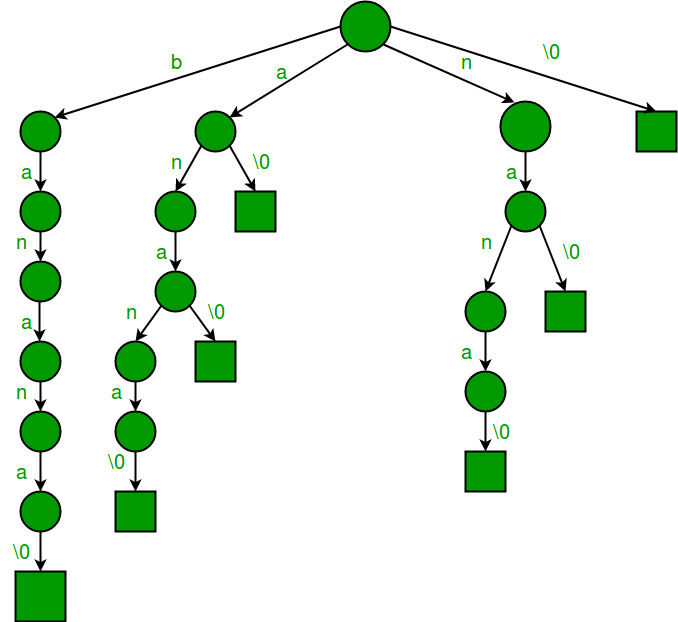
\includegraphics[width=17cm, height=9cm]{a3.png}
    \caption{Creation of Trie}
    \label{fig:StoringExample}
\end{figure}
If we join chains of single nodes, we get the following compressed trie, which is the Suffix Tree for given text “banana\textbackslash0” 
\begin{figure}[H]
    \centering
    \includegraphics[width=17cm, height=9cm]{a4.png}
    \caption{Creation of Suffix Tree by compressing Trie}
    % \label{fig:StoringExample}/
\end{figure}
\textbf{How to search a pattern in the built suffix tree? }
\\
1. Starting from the first character of the pattern and root of the Suffix Tree, do the following for every character:
\\
 For the current character of the pattern, if there is an edge from the current node of suffix tree, follow the edge.
\\
 If there is no edge, print “pattern doesn’t exist in the text” and return.
\\
2. If all characters of pattern have been processed, i.e., there is a path from root for characters of the given pattern, then print “Pattern found”. Let us consider the example pattern as “nan” to see the searching process. Following diagram shows the path followed for searching “nan” or “nana”.
\\
Every pattern that is present in text (or we can say every substring of text) must be a prefix of one of all possible suffixes.

\section{Knuth–Morris–Pratt algorithm}
\label{sec:KMP algorithm}
The KMP matching algorithm uses degenerating property (pattern having the same sub-patterns appearing more than once in the pattern) of the pattern and improves the worst-case complexity to O(n+m).
\\
The basic idea behind KMP’s algorithm is: whenever we detect a mismatch (after some matches), we already know some of the characters in the text of the next window. We take advantage of this information to avoid matching the characters that we know will anyway match. 
\\

\begin{figure}[H]
    \centering
    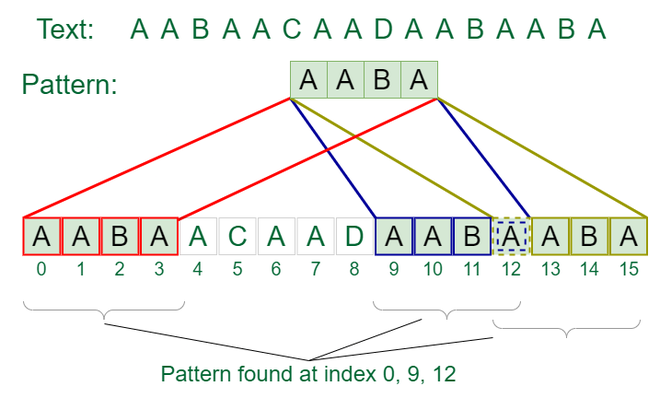
\includegraphics[width=14cm, height=9cm]{kmp_algorithm.png}
    \caption{Pattern searching using KMP's algorithm}
    \label{fig:StoringExample}
\end{figure}

\\
\textbf{Preprocessing overview}
\\
• KMP algorithm preprocesses pat[] and constructs an auxiliary lps[] of size m (same as the size of the pattern) which is used to skip characters while matching.
\\
• Name lps indicates the longest proper prefix which is also a suffix. A proper prefix is a prefix with a whole string not allowed. For example, prefixes of “ABC” are “”, “A”, “AB” and “ABC”. Proper prefixes are “”, “A” and “AB”. Suffixes of the string are “”, “C”, “BC”, and “ABC”.
\\
• We search for lps in subpatterns. More clearly we focus on sub-strings of patterns that are both prefix and suffix.
\\
• For each sub-pattern pat[0..i] where i = 0 to m-1, lps[i] stores the length of the maximum matching proper prefix which is also a suffix of the sub-pattern pat[0..i].
\\
\\
\textbf{Preprocessing algorithm}
\\
• We calculate values in lps[]. To do that, we keep track of the length of the longest prefix suffix value (we use len variable for this purpose) for the previous index
\\
• We initialize lps[0] and len as 0.
\\
• If pat[len] and pat[i] match, we increment len by 1 and assign the incremented value to lps[i].
\\
• If pat[i] and pat[len] do not match and len is not 0, we update len to lps[len-1]

\begin{algorithm}[H]
\caption*{KMP algorithm}
\label{spapsuedocode}
\begin{algorithmic}
\STATE 1. We start the comparison of pat[j] with j = 0 with characters of the current window of text.
\STATE 2. We keep matching characters txt[i] and pat[j] and keep incrementing i and j while pat[j] and txt[i] keep matching.
\STATE 3. When we see a mismatch
\STATE \hspace{1cm}  We know that characters pat[0..j-1] match with txt[i-j…i-1] (Note that j starts with 0 and increments it only when there is a match).
\STATE \hspace{1cm} We also know (from the above definition) that lps[j-1] is the count of characters of pat[0…j-1] that are both proper prefix and suffix.
\end{algorithmic}
\end{algorithm}

\section{Finite Automata algorithm}
\label{sec:Finite Automata algorithm}
1. Idea of this approach is to build finite automata to scan text T for finding all occurrences of pattern P.
2. This approach examines each character of text exactly once to find the pattern. Thus it takes linear time for matching but preprocessing time may be large.
3. It is defined by tuple M = {Q, \begin{math}\sum\end{math}, q, F, \begin{math}\sigma\end{math}} 
\\
Where Q = Set of States in finite automata
\\
\begin{math}\sum\end{math}=Sets of input symbols
\\
q = Initial state
\\
F = Final State
\\
\begin{math}\sigma\end{math} = Transition function
\\
Time Complexity = O(M³|\begin{math}\sum\end{math}|)

A finite automaton M is a 5-tuple (Q, q0,A,\begin{math}\sum\end{math},\begin{math}\delta\end{math}), where

Q is a finite set of states,
q0 \begin{math}\epsilon\end{math} Q is the start state,
A subset of Q is a notable set of accepting states,
\begin{math}\sigma\end{math} is a finite input alphabet,
\begin{math}\delta\end{math} is a function from Q x \begin{math}\sigma\end{math} into Q called the transition function of M.
\\
The finite automaton starts in state q0 and reads the characters of its input string one at a time. If the automaton is in state q and reads input character a, it moves from state q to state \begin{math}\delta\end{math} (q, a). Whenever its current state q is a member of A, the machine M has accepted the string read so far. An input that is not allowed is rejected.
\\
A finite automaton M induces a function \begin{math}\phi\end{math} called the called the final-state function, from \begin{math}\epsilon\end{math}* to Q such that \begin{math}\phi\end{math}(w) is the state M ends up in after scanning the string w. Thus, M accepts a string w if and only if \begin{math}\phi\end{math}(w) \begin{math}\epsilon\end{math} A.

\begin{algorithm}[H]
\caption*{Finite automata algorithm}
\label{psuedocode}
\begin{algorithmic}
\STATE FINITE AUTOMATA (T, P)
\STATE State <- 0
\STATE for l <- 1 to n
\STATE State <- \begin{math}\delta\end{math}(State, ti)
\STATE If State == m then
\STATE Match Found
\STATE else
\STATE end
\end{algorithmic}
\end{algorithm}

\begin{figure}[H]
    \centering
    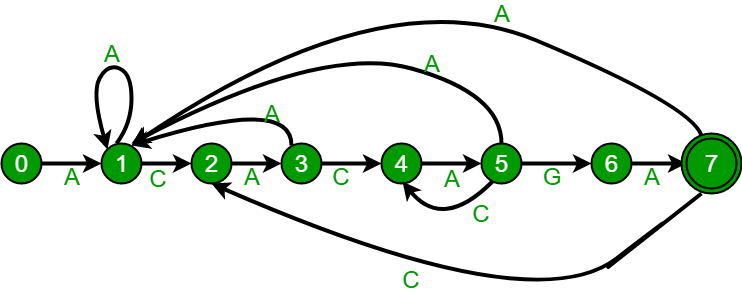
\includegraphics[width=16cm, height=8cm]{finiteauto1.png}
    \label{fig:StoringExample}
\end{figure}

\begin{figure}[H]
    \centering
    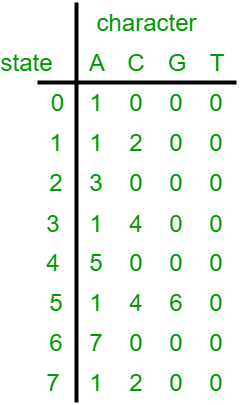
\includegraphics[width=10cm, height=12cm]{finiteauto2.png}
    \caption{Finite automation for ACACAGA pattern}
    \label{fig:StoringExample}
\end{figure}


\section{Aho-Corasick Algorithm}
Given an input text and an array of k words, arr[], find all occurrences of all words in the input text. Let n be the length of text and m be the total number of characters in all words, i.e. m = length(arr[0]) + length(arr[1]) + … + length(arr[k-1]). Here k is total numbers of input words.
\\
If we use a linear time searching algorithm like KMP, then we need to one by one search all words in text[]. This gives us total time complexity as O(n + length(word[0]) + O(n + length(word[1]) + O(n + length(word[2]) + … O(n + length(word[k-1]). This time complexity can be written as O(n*k + m). 
\\
\textbf{Aho-Corasick} Algorithm finds all words in O(n + m + z) time where z is total number of occurrences of words in text. 
\\
\\
\section*{Algorithm Overview}

This algorithm is a \textbf{preprocessing} approach that processes the text in three main components:

\begin{enumerate}
    \item \textbf{Go To:}  
    This function follows the edges of a Trie constructed from all words in \texttt{arr[]}. Represented as a 2D array $g[][]$, it stores the next state for a given state and character.
    
    \item \textbf{Failure:}  
    This function manages the fallback edges when the current character lacks a direct edge in the Trie. Represented as a 1D array $f[]$, it stores the next state for each state when no matching edge exists.

    \item \textbf{Output:}  
    Contains indexes of all words that end at the current state, stored in a 1D array $o[]$ as a bitmap indicating all matches for a given state.
\end{enumerate}

\section*{Preprocessing the Text to Generate Automaton}
\begin{itemize}
    \item Build a Trie (or Keyword Tree) for all words, filling entries in the \texttt{goto} array $g[][]$ and \texttt{output} array $o[]$.
    \begin{figure}[H]
    \centering
    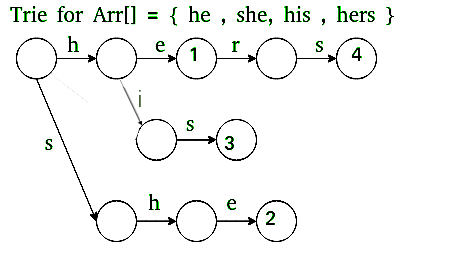
\includegraphics[width=12cm, height=8cm]{aho1.png}
    \caption{Trie}
    \end{figure}
    \item Extend the Trie into an automaton to enable linear-time matching, filling entries in the \texttt{failure} array $f[]$ and updating \texttt{output} $o[]$.
    \begin{figure}[H]
    \centering
    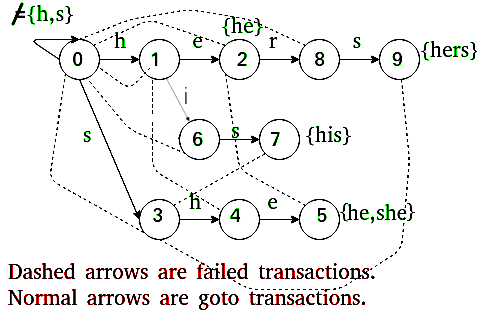
\includegraphics[width=14cm, height=10cm]{aho2.png}
    \caption{Automaton}
    \end{figure}
\end{itemize}

\subsection*{Detailed Steps}

\paragraph{Go To:}  
Construct the Trie. For characters lacking an edge at the root, add an edge back to the root.

\paragraph{Failure:}  
For each state $s$, find the longest proper suffix that is also a prefix of a pattern using a Breadth-First Traversal (BFS) of the Trie.

\paragraph{Output:}  
Store indexes of all words ending at each state $s$ as a bitwise map (by performing bitwise OR operations). This is also computed using BFS with Failure.

\paragraph{Matching:}  
Traverse the given text over the built automaton to locate all matching words.
\\

\section{Application}
\subsection{General Applications}
\textbf{Text Searching and Information Retrieval:} Pattern searching algorithms are fundamental in information retrieval systems, such as search engines, where they help users find relevant documents, web pages, or content based on search queries or keywords.
\\
\textbf{Data Mining and Text Analysis:} In data mining and text analysis, pattern searching is essential for extracting meaningful information from large datasets, including text data. This is used in sentiment analysis, topic modeling, and identifying trends.
\\
\textbf{Genomics and Bioinformatics:} Pattern searching is crucial in analyzing DNA and protein sequences, finding specific motifs, detecting gene sequences, and identifying mutations or variations in biological data.
\\
\textbf{Text Compression:} Pattern searching can be used in text compression techniques, such as finding repeated patterns to compress text more efficiently.
\\
\textbf{Network Security:} Intrusion detection systems and network security applications use pattern searching algorithms to identify known attack patterns or suspicious network activities in log files and network traffic.
\\
\textbf{Image Processing:} In image processing, pattern matching is used for object recognition, image retrieval, and locating specific features within images.
\\
\textbf{Spell Checkers and Autocorrection: } Spell checkers and autocorrection systems use pattern searching to identify misspelled words and suggest corrections based on similar patterns.
\\
\textbf{File and Text Editing:} Text editors and search tools often employ pattern searching algorithms to help users locate and edit text within documents or source code.
\subsection{Technique Specific Applications}
\begin{itemize}
    \item \textbf{Trie}
    \begin{itemize}
        \item \textbf{Search Engines}: Tries are used for autocomplete suggestions and predictive text by organizing and retrieving stored words based on prefixes.
        \item \textbf{IP Routing}: In network routing, Tries store IP addresses and optimize routing paths.
        \item \textbf{Spell Checkers}: Tries provide efficient spell correction and autocorrect by quickly checking for word presence or suggesting alternatives.
    \end{itemize}

    \item \textbf{Suffix Trees}
    \begin{itemize}
        \item \textbf{Genomics}: Suffix trees are used in DNA sequence alignment, allowing for rapid searches of genetic patterns within large genomes.
        \item \textbf{Plagiarism Detection}: They help identify matching sequences between documents by efficiently finding repeated or similar phrases.
        \item \textbf{Data Compression}: Suffix trees are instrumental in detecting repeating substrings, which is crucial in compression algorithms like Lempel-Ziv.
    \end{itemize}

    \item \textbf{Knuth-Morris-Pratt (KMP) Algorithm}
    \begin{itemize}
        \item \textbf{Word Processing Applications}: Employed for find-and-replace functions by efficiently locating patterns within text.
        \item \textbf{Bioinformatics}: Facilitates search for specific gene sequences or motifs in DNA strands.
        \item \textbf{Intrusion Detection Systems}: Used to detect known signatures or patterns in network traffic, ensuring quick threat detection.
    \end{itemize}

    \item \textbf{Finite Automata}
    \begin{itemize}
        \item \textbf{Lexical Analysis in Compilers}: Matches keywords and tokens in source code by using state transition models.
        \item \textbf{Speech Recognition}: Matches audio input to known phoneme sequences or words, aiding in interpreting continuous speech.
        \item \textbf{Text Editors}: Enables fast search and navigation through patterns within large documents.
    \end{itemize}

    \item \textbf{Aho-Corasick Algorithm}
    \begin{itemize}
        \item \textbf{Web Content Filtering}: Blocks or flags inappropriate content by searching for a set of banned words across web pages.
        \item \textbf{Spam Detection}: Detects specific keywords within email content that match spam patterns, providing real-time filtering.
        \item \textbf{Digital Forensics}: Locates critical evidence across large data sets by searching for multiple keywords simultaneously.
    \end{itemize}
\end{itemize}

\section{Complexity Analysis}
We have conducted a complexity analysis for each pattern searching technique utilized in our project. Let:
\begin{itemize}
    \item \( n \) = length of the given text file
    \item \( m \) = length of the pattern to be searched
    \item \( l \) = average length of each line in the text file
\end{itemize}

\subsection{Trie}
\begin{itemize}
    \item \textbf{Space Complexity:} \( O(n^2) \) due to the formation of the trie from preprocessing the text file.
    \item \textbf{Time Complexity:} \( O(n^2) \), dominated by trie creation; pattern searching takes \( O(m) \).
\end{itemize}

\subsection{Suffix Tree (Naive Approach)}
\begin{itemize}
    \item \textbf{Space Complexity:} In the worst case, for a string with all unique characters, the suffix tree could have \( O(n^2) \) nodes, as each suffix could lead to a new node. In the average case, it could be \( O(n \cdot l) \).
    \item \textbf{Time Complexity:} Building the suffix tree takes \( O(n \cdot l^2) \); searching the pattern takes \( O(m) \).
\end{itemize}

\subsection{KMP Algorithm}
\begin{itemize}
    \item \textbf{Space Complexity:} \( O(n) \)
    \item \textbf{Time Complexity:} \( O(n + m) \)
\end{itemize}

\subsection{Finite Automata}
\begin{itemize}
    \item \textbf{Space Complexity:} \( O(n \cdot l + m \cdot 256) \approx O(n) \)
    \item \textbf{Time Complexity:} \( O(n \cdot l + m \cdot 256) \approx O(n) \)
\end{itemize}

\subsection{Aho-Corasick Algorithm}
\begin{itemize}
    \item \textbf{Space Complexity:} \( O(m) \)
    \item \textbf{Time Complexity:} \( O(m + n) \)
\end{itemize}

\subsection{Performance Graphs}
\begin{figure}[H]
    \centering
    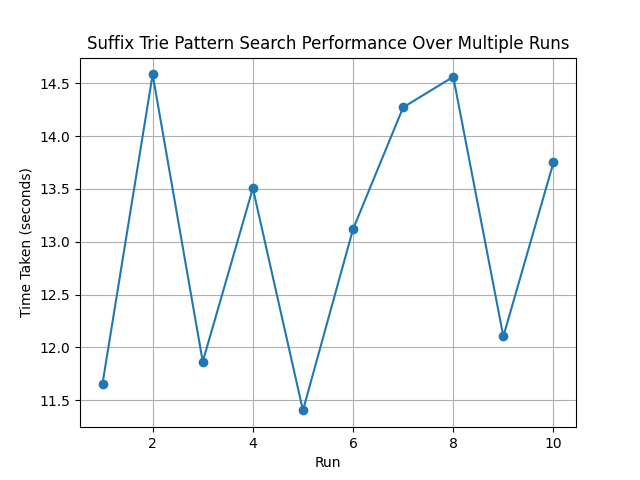
\includegraphics[width=12cm, height=8cm]{time_trie.png}
    \caption{Performance of the Trie Algorithm}
\end{figure}

\begin{figure}[H]
    \centering
    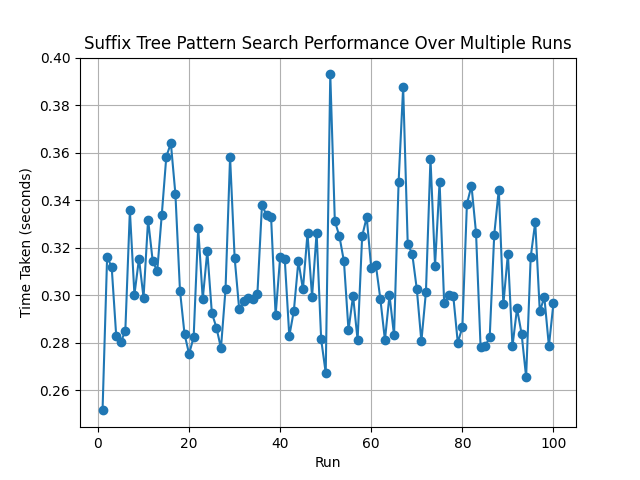
\includegraphics[width=12cm, height=8cm]{time_Naive.png}
    \caption{Performance of the Suffix Tree (Naive Approach)}
\end{figure}

\begin{figure}[H]
    \centering
    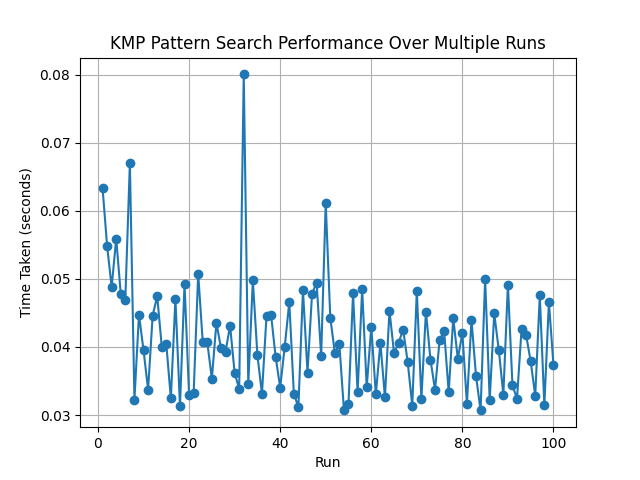
\includegraphics[width=12cm, height=8cm]{time_KMP.png}
    \caption{Performance of the KMP Algorithm}
\end{figure}

\begin{figure}[H]
    \centering
    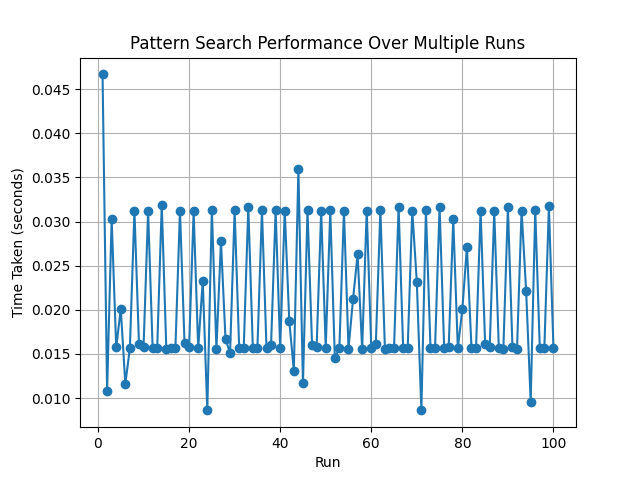
\includegraphics[width=12cm, height=8cm]{time_FA.png}
    \caption{Performance of the Finite Automata Algorithm}
\end{figure}

\begin{figure}[H]
    \centering
    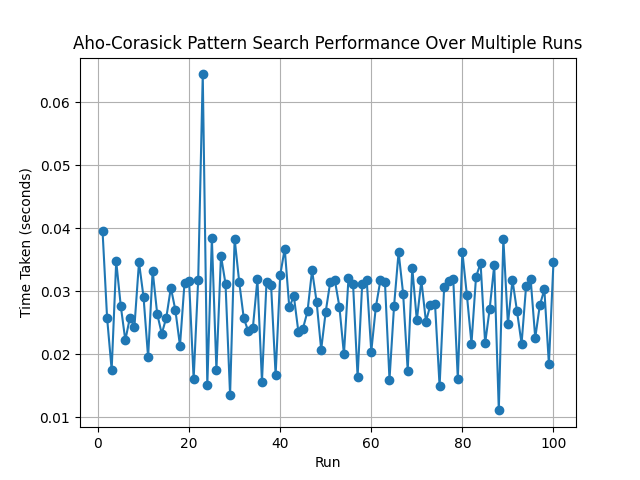
\includegraphics[width=12cm, height=8cm]{time_modifiedTrie.png}
    \caption{Performance of the Aho-Corasick Algorithm}
\end{figure}

    
\section{Conclusion}
\label{sec:conc}
In conclusion, the project on string pattern searching has provided us with a comprehensive understanding of the techniques, algorithms, and applications associated with this fundamental concept in computer science. Throughout this endeavor, we have explored a range of string searching algorithms, Knuth-Morris-Pratt, Finite automata, and more, each with its unique advantages and trade-offs. We have witnessed how string pattern searching plays a pivotal role in various domains. Furthermore, we have delved into the underlying data structures, like suffix trees. \\
Each method offers unique strengths: Tries for prefix searches, Suffix Trees for full-text searches, KMP and Finite Automata for efficient single-pattern matching, and Aho-Corasick for multi-pattern searches. Together, these methods provide scalable, adaptable solutions for diverse text-searching requirements.



\section{Bibliography and Citations}
\label{sec:biblio}

\href{https://www.geeksforgeeks.org/aho-corasick-algorithm-pattern-searching/}{Aho-Corasick Algorithm}

\href{https://www.geeksforgeeks.org/pattern-searching-using-suffix-tree/}{Suffix tree}

\href{https://www.geeksforgeeks.org/pattern-searching-using-trie-suffixes/}{Tries}

\href{https://www.geeksforgeeks.org/kmp-algorithm-for-pattern-searching/}{KMP Algorithm}

\href{https://www.geeksforgeeks.org/finite-automata-algorithm-for-pattern-searching/}{Finite Automata algorithm}

\section{References}
\label{sec:refrnces}

CTAN. BiBTeX documentation.
\\
Leslie Lamport. LaTeX: A Document Preparation System. Pearson Education India, 1994.
\\
Thomas H. Cormen(CLRS). Introduction to algorithm.\emph{ Library of Congress Cataloging-in-Publication}. 1990

\end{document}